The Hausdorff measure generalizes the notion of measure for lower-dimensional
objects in a higher-dimensional space or even in an arbitrary metric space.
The idea is essentially similar to the construction of Lebesgue measure, and
the general case is called the Carathéodory construction. The difference is
that we measure sets by their diameter, attributing to each an s-dimensional
"volume" based on its diameter raised to the power of s. For this construction,
we define a cover of E by sets of diameter less than δ as a δ-cover of E. And
we consider only countable covers. We note that
\[\mathcal{H}_\delta^s(E)=\inf_{C}\sum_{I\in C}\omega_s\left(\frac{\text{diam}(I)}{2}\right)^s\]
where $s\in\mathbb{R}_{\geq 0}$ is a dimension, $\omega_s\in\mathbb{R}$ is a
coefficient, preferably continuous or smooth as a function of $s$, and $C$ is a
$\delta$-cover of $E$. We may assume that
\[\omega_s = \frac{\pi^{s/2}}{\Gamma(1+s/2)}\]
We define the Hausdorff measure as a limit of the previous value. It exists
because $\mathcal{H}_\delta^s(E)$ is an increasing function of $\delta$. We note
\[\mathcal{H}^s(E)=\lim_{\delta\rightarrow0^+}\mathcal{H}^s_\delta(E)\]

I shall introduce the notion of $s$-variation of a cover $S$ as
\[\text{Var}^s(S)=\sum_{I\in S}\omega_s\left(\frac{\text{diam}(I)}{2}\right)^s\]

\textbf{Proposition:} \textbf{For a natural $n\geq 0$, $\omega_n$ is a volume of a unit
$n$-dimensional ball.}
\vspace{1ex}

\subsection{Properties of Hausdorff measure}

\textbf{Proposition:} \textit{Hausdorff measure is a Borel measure.}

\vspace{2ex}
\textbf{Proposition:} $\mathcal H^0$ is the counting measure.

\vspace{2ex}
\textbf{Proposition:} \textit{In the definition of Hausdorff measure we can consider
only closed or open sets.}

\vspace{2ex}
\textbf{Proposition:} \textit{Hausdorff measure of dimension $m\in N$ coincide on
$m$-dimensional affine subspaces with their Lebesgue measure.}

\vspace{2ex}
\textbf{Proposition:} \textit{The $n$-dimetional Hausdorff measure traced to a
$n$-dimentional $\mathcal{C}^1$-submanifold of $R^m$ induces the area measure
on this submanifold and coincides with the integral measure via parametrisation
on it.}

\vspace{2ex}
\textbf{Proposition:} \textit{A restriction of $\mathcal H^s$ on a locally
$\mathcal H^s$-finite set is a Radon measure.}

\vspace{1ex}
\textbf{Remark:} Proofs to those proposition can be found in the book "Geometric
measure theory" be Francesco Maggi \cite{maggi}.

\vspace{2ex}
\textbf{Definition:} \textit{Let $E$ be a Borel subset of a metric space $X$.
The \textbf{upper $d$-dimensional density} (with respect to $\mathcal H^d$) of $E$ at
the point $x$ is defined by setting
\[\Theta^*_d(E,x)=\limsup_{r\rightarrow 0}\frac{\mathcal H^d(E\cap B_c(x,r))}{\omega_dr^d}\]}

\vspace{2ex}
\textbf{Theorem:} \textit{Let $E$ be a Borel subset of a metric space $X$, and
assume that $E$ is locally $\mathcal H^d$-finite. Then the following properties
hold true:
\begin{enumerate}
    \item The upper density of external points is almost everywhere zero,
        $\Theta^*_d(E, x)=0$ for $\mathcal H^d$-almost every $x\in E^c$.
    \item The upper density is bounded from below, $\frac{1}{2^d}\leq\Theta^*
        _d(E,x)$ for $\mathcal H^d$-almost every $x\in E^c$.
    \item If $X\cong\mathbb R^n$, then the upper density is bounded from above
        by 1, $\Theta^*_d(E,x)\leq 1$ for $\mathcal H^d$-almost every $x\in E$.
    \item If $X$ is a generic metric space, then the upper density is bounded
        from above by a slightly different constant, $\Theta^*_d(E,x)\leq3^d$
        for $\mathcal H^d$-almost every $x\in E$.
\end{enumerate}
}

\vspace{1ex}
\textbf{Proof:} Proofs of propositions 2-3 can be found in \cite{giovanni_alberti}
on page 48.

\vspace{1ex}
\begin{enumerate}
    \item The core of this proof relies on the regularity of $\mu:=\mathcal H^d\,
        \llcorner E$ and Vitali's Covering Lemma. We define $E_t:=\{x\in E^c\,|\,\Theta^*_d(E,x)>t\}$
        and aim to prove that it is $\mathcal H^d$-null for $t>0$. From the
        definition of $E_t$ we know that $E$ is highly concentrated around the
        points of $E_t$. This effectively allows us to reduce the study of $E_t$ to
        the study of appropriate covers. Let $A\supseteq E_t$ be an open neighborhood of $E_t$.
        We then consider the family of closed balls $\mathcal F:=\{\overline{B(x,r)}\subset A\,|\,x\in E_m\;\&
        \;\mathcal H^d(\overline{B(x,r)}\cap E)>t\omega_dr^d\}$. Within this family,
        we can consider balls of diameter $<1$. Then for \textbf{Vitali's
        Covering Lemma} we can choose a dilation coefficient $k\in(3,+\infty)$
        and we fix ball dilatation procedure with coefficient $k$ by $B\mapsto
        \widehat B$. Lemma provides a disjoint subfamily $\mathcal G$ such that
        the delated by $\widehat\cdot$ balls cover $E_t$. We then have the following
        inequality
        \begin{align*}
            \mu(A)\geq\sum_{B\in\mathcal G}\mu(B)\geq t\omega_d\sum_{B\in
            \mathcal G}r(B)^d=\frac{t}{k^d}\omega_d\sum_{B\in\mathcal G}r(
            \widehat B)^d\geq\frac{t}{k^d}\mathcal H^d_1(E_n)
        \end{align*}
        Since $\mu(A)$ can be chosen arbitrary small, it follows that $\mathcal
        H^d_1(E_t)=0$ and consequently $\mathcal H^d(E_t)=0$.
    \item \cite{giovanni_alberti}
    \item \cite{giovanni_alberti}
    \item If we follow a similar construction to the proof of the first
        proposition for a set $E_t:=\{x\in E\,|\,\Theta^*_d(E,x)>t\}$, then
        we arrive at
        \[\mathcal H^d(E_m)\geq\frac{t}{k^d}\mathcal H^d(E_m)\]
        and if $t>k^d$ we get $\mathcal H^d(E_m)=0$, and as it is true for all
        $k>3$, we have $\Theta^*_d(E,x)\leq3^d$. It's worth noticing that usually there
        are no generalisation in Vitali's lemma and one usually proves for 5
        instead of 3.
\end{enumerate}

\subsection{Hausdorff dimension}
To a set $S$ we can associate a number $s=\text{inf}\{a\geq 0\,|\,\mathcal{H}^a
(S)=0\}$. It's called its Hausdorff dimension.

\vspace{2ex}
\textbf{Proposition:} \textit{If $E\subseteq\mathbb R$ then $\dim(E)\in [0, n]$.
Moreover $\mathcal H^s(E)=\infty$ for every $s<\dim(E)$ and $\mathcal H^S(E)\in
(0,\infty)$ implies $s=\dim(E)$.}

\vspace{2ex}
\textbf{Proposition:} \textit{If $A$ is an open set in $\mathbb R^n$, then $\dim
(A) = n$.}

\vspace{2ex}
\textbf{Proposition:} \textit{For a Lipschitz function $f:\mathbb{R}^n\rightarrow
\mathbb{R}^m$ we have the following inequality
\[ \mathcal{H}^s(f[E])\leq\text{Lip}(f)^s\mathcal{H}^s(E) \]
for every $s>0$ and $E\subseteq\mathbb{R}^n$ and $\text{dim}(E)<\text{dim}(f[E])$.}

\subsection{Dimension of cantor sets}
Here we compute the dimension of generalized set. Let $n\in\mathbb{N}$ and
$m\in\mathbb{N}^*$ so that $2m<n$. Then we can define $C_k$ ($k\in\mathbb{N}$)
define recursively by agreeing that $C_0=\{[0,1]\}$ and we obtain $C_{k+1}$ from $C_k$
by cutting out the open middle part from each segment of $C_k$ and living side parts
of length $m/n$ of original interval. We will note $C=\lim C_k=\bigcap C_k$.
\begin{center}
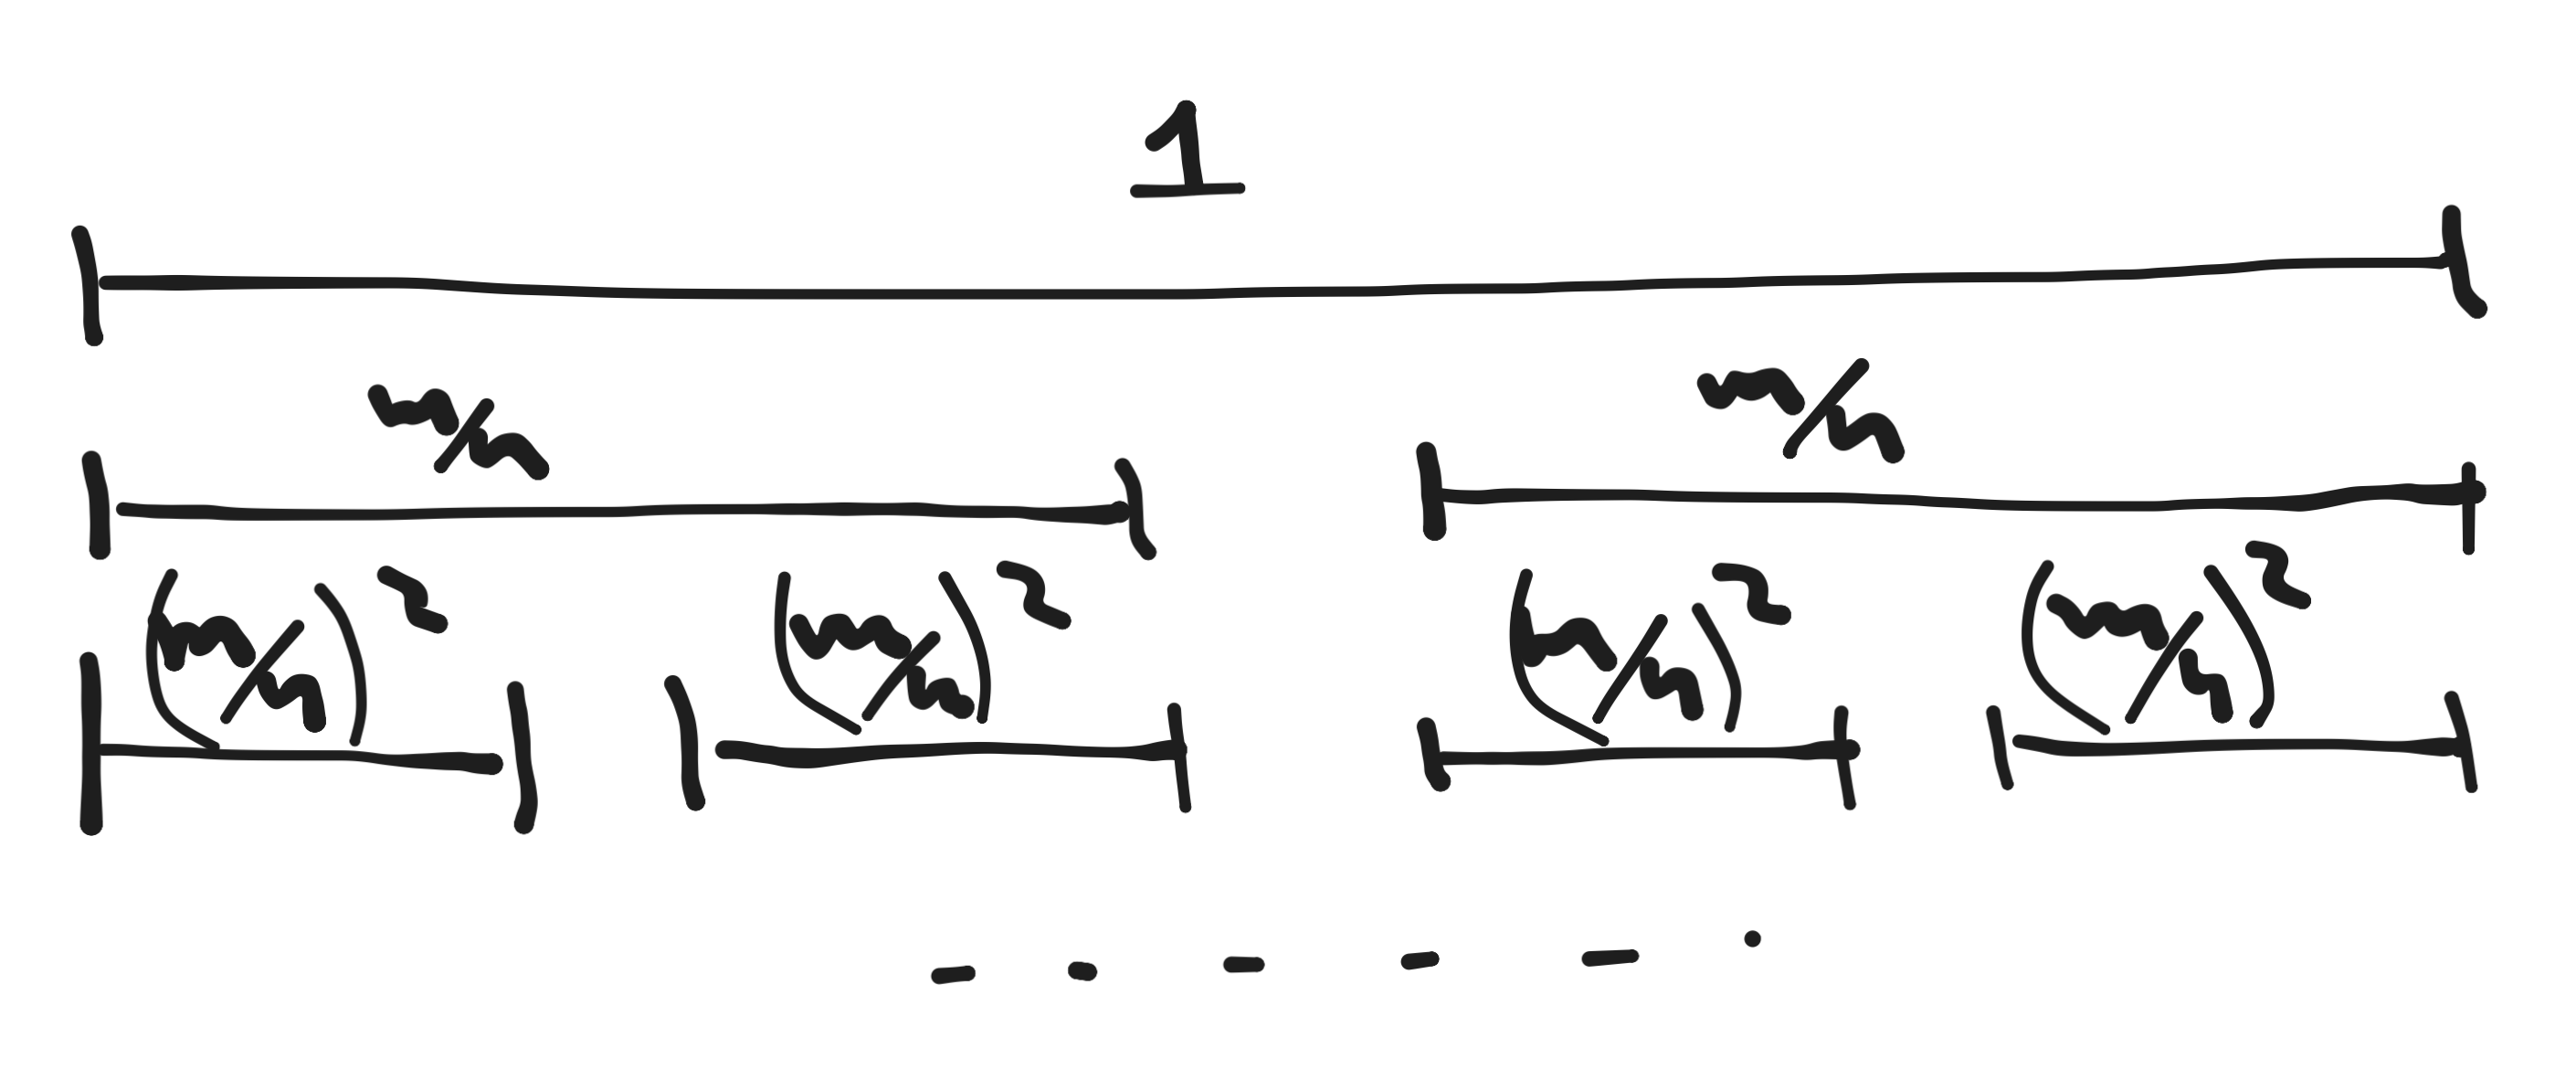
\includegraphics[scale=0.15]{cantor.png}
\end{center}
Obviously $C_k$ is a $(m/n)^k$-cover of $C$, so
\[ \mathcal{H}_{(m/n)^k}^s \leq \sum_{I\in C_k}\omega_s(\frac{\text{diam}(I)}{2})^s
=\omega_s2^k((m/n)^k)/2)^s=\omega_s/2^s(2(m/n)^s)^k \]
And if $s>\text{log}_{n/m}(2)$ we have right side approaching 0 as $k$ tends to
infinity. That means that $\text{dim}(C)\leq\text{log}_{n/m}(2)$.


Now we need to prove the inequality in the other direction. Let $s=\text{log}_
{n/m}(2)$. And let $S$ be a $(m/n)^k$-cover of $C$. In fact by the construction
$C$ is an intersection of compacts on a real line, so is compact. And by one of
the previous propositions we can conceder only open covers. Then by compactness 
we can leave only a finite number of sets in $S$ and this way we reduce its 
Hausdorff variance and we can extend the resting elements to closed intervals
of the same diameter. This does not change the variance. The new cover is noted
by $S'$. Now in every interval of $S'$ we can find 2 maximal intervals from some
$C_i$ and $C_j$, so the they are disjoint. If we can't do that, then there are no points
of $C$ in this interval and we can throw away that set also. So now we have 2 
maximal intervals $J$ and $J'$ in $I$. They are ordered. Between them we
have an interval $K$ and as they are maximal $I\setminus J\setminus K\setminus J'$ does not contain
any points from $C$ and we can through those parts away from the covering.
By the construction
\[|J|,|J'|\leq \frac{m}{n}\cdot \frac{n}{n-2m}|K|=\frac{m}{n-2m}|K|\]
Now we have $1/2(|J|+|J'|) \leq \frac{m}{n-2m}|K|$
\[|I|^s=(|J|+|J'|+|K|)^s\geq((1+\frac{n-2m}{2m}))(|J|+|J'|))^s=(\frac{n}{m}1/2(|J|+|J'|))^s=2(1/2(|J|+|J'|))^s\geq|J|^s+|J'|^s\]
Where the last step is done by concavity of function $x\mapsto x^s$.
That means that we can reduce this any cover to a $C_k$ cover which has a
smaller $s$-variation. That means that for dimension $s=\text{log}_{n/m}(2)$
the $\mathcal{H}^s(C)$ is finite as the $s$-variation of $C_k$ is always $
\omega_s/2^s$.

\vspace{1ex}
\textbf{Remark:} This is a variation on the proof given in the book "The geometry
of fractal sets" by K. J. Flaconer, generelised to the case of arbitrary $m$ and
$n$. In this book the proof is done for the case $m=1$, $n=3$.

\vspace{1ex}
\textbf{Proposition:} \textit{There is a subset of $[0,1]$ with а Hausdorff dimension
$1$, but Lebesgue measure 0.}

\vspace{1ex}
To show that we shall use Cantor's sets. Let $C_{m/n}$ be a set discussed in a
previous paragraph. Then $S=\bigcap C_{m/(2m+1)}$ is a set of dimension $1$. As
for every $0\leq s<1$ there is such $m$, that $\text{log}_{n/m}(2)=\text{log}_{
(2m+1)/m}(2)>s$, as $\text{log}_{(2m+1)/m}(2)\rightarrow 1$. And thus $\mathcal
{H}^s(S)>\mathcal{H}^s(C_{m/(2m+1)})=\infty$.
